\documentclass[tikz,border=2pt]{standalone}
\usepackage{tikz}
\usetikzlibrary{
  arrows.meta,
  calc,
  decorations.markings,
  decorations.pathmorphing,
  decorations.pathreplacing,
  fit,
  patterns,
  positioning,
  shapes.arrows,
  shapes.geometric,
  shapes.misc,
  shapes.symbols,
  through,
  intersections,
  matrix,
  backgrounds,
  cd
}
\usepackage{amsmath,amssymb}
\usepackage{xcolor}
% Site-wide TikZ colour palette. Keep these in sync with preface.tex
% style; new entries can use these names directly.
\definecolor{winered}{HTML}{8B1A1A}
\definecolor{prussianblue}{HTML}{003366}
\definecolor{agreen}{HTML}{2A6E3F}
\definecolor{oxblue}{HTML}{002147}
\definecolor{burntorange}{HTML}{B8541D}

\begin{document}
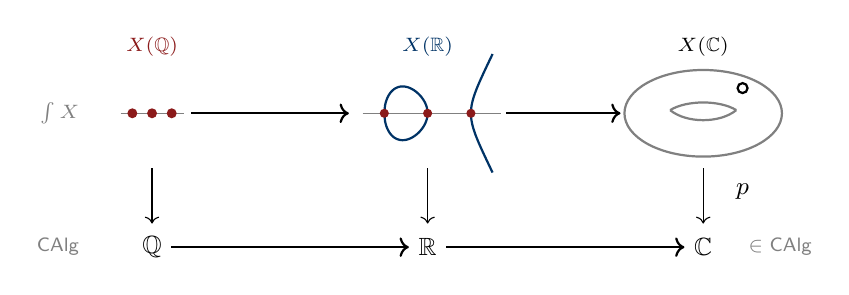
\begin{tikzpicture}
% X(Q): three winered points
\node[font=\scriptsize, winered, anchor=south] at (-3.5, 0.6) {$X(\mathbb{Q})$};
\draw[thin, gray] (-3.9, 0) -- (-3.1, 0);
\fill[winered] (-3.75, 0) circle (1.8pt);
\fill[winered] (-3.5,  0) circle (1.8pt);
\fill[winered] (-3.25, 0) circle (1.8pt);

% X(R): real curve with X(Q) marked
\node[font=\scriptsize, prussianblue, anchor=south] at (0, 0.6) {$X(\mathbb{R})$};
\begin{scope}[shift={(0, 0)}, scale=0.55]
  \draw[thin, gray] (-1.5, 0) -- (1.7, 0);
  \draw[thick, prussianblue, domain=-1:0, samples=60, smooth]
    plot (\x, { sqrt((\x)*(\x)*(\x) - (\x)) });
  \draw[thick, prussianblue, domain=-1:0, samples=60, smooth]
    plot (\x, { -sqrt((\x)*(\x)*(\x) - (\x)) });
  \draw[thick, prussianblue, domain=1:1.5, samples=60, smooth]
    plot (\x, { sqrt((\x)*(\x)*(\x) - (\x)) });
  \draw[thick, prussianblue, domain=1:1.5, samples=60, smooth]
    plot (\x, { -sqrt((\x)*(\x)*(\x) - (\x)) });
  \fill[winered] (-1, 0) circle (3pt);
  \fill[winered] ( 0, 0) circle (3pt);
  \fill[winered] ( 1, 0) circle (3pt);
\end{scope}

% X(C): plain torus with one puncture
\node[font=\scriptsize, anchor=south] at (3.5, 0.6) {$X(\mathbb{C})$};
\begin{scope}[shift={(3.5, 0)}]
\draw[thick, gray] (0, 0) ellipse (1.0 and 0.55);
\draw[thick, gray]
  (-0.42, 0.04) .. controls (-0.21, -0.13) and (0.21, -0.13) .. (0.42, 0.04);
\draw[thick, gray]
  (-0.42, 0.04) .. controls (-0.21,  0.17) and ( 0.21, 0.17) .. (0.42, 0.04);
\draw[thick, fill=white] (0.5, 0.32) circle (1.8pt);
\end{scope}

% horizontal functoriality arrows
\draw[->, thick] (-3.0, 0) -- (-1.0, 0);
\draw[->, thick] ( 1.0, 0) -- ( 2.45, 0);

% vertical p arrows
\foreach \x in {-3.5, 0, 3.5} {
  \draw[->, thin] (\x, -0.7) -- (\x, -1.4);
}
\node[font=\small] at (4.0, -1) {$p$};

% base row
\node[font=\small] (Qr) at (-3.5, -1.7) {$\mathbb{Q}$};
\node[font=\small] (Rr) at ( 0,   -1.7) {$\mathbb{R}$};
\node[font=\small] (Cr) at ( 3.5, -1.7) {$\mathbb{C}$};
\draw[->, thick] (Qr) -- (Rr);
\draw[->, thick] (Rr) -- (Cr);
\node[font=\scriptsize, gray, anchor=west] at (3.95, -1.7) {$\in \mathsf{CAlg}$};

% side labels
\node[font=\scriptsize, gray, anchor=east] at (-4.3,  0)   {$\int X$};
\node[font=\scriptsize, gray, anchor=east] at (-4.3, -1.7) {$\mathsf{CAlg}$};
\end{tikzpicture}
\end{document}
